\documentclass[12pt, a4paper]{article}
\usepackage[utf8]{inputenc}
\usepackage{appendix}
\usepackage{graphicx}
\usepackage{enumerate}
\usepackage{subfig}
\usepackage{float}
\usepackage{indentfirst}
\usepackage{amsmath}
\usepackage{amsfonts}
\usepackage{geometry}   %设置页边距的宏包
\usepackage{titlesec}   %设置页眉页脚的宏包
\usepackage{enumitem}
\usepackage{booktabs}
\usepackage[section]{placeins}
\geometry{left=2.54cm,right=2.54cm,top=2.54cm,bottom=2.54cm}


\begin{document}

\pagestyle{plain}

\begin{titlepage}

	\begin{center}	
	% Title

	\vspace{10ex}

	\hrule

	\vspace{2ex}

	\textbf{\Large{UM-SJTU} \Large{J}\large{oint} \Large{I}\large{nstitute} \\
	\Large{P}\large{HYSICS} \Large{L}\large{ABORATORY} \\
	\large{(}\Large{V}\large{P241)}}\\
	
	\vspace{2ex}

	\hrule
	
	\vspace{25ex}
	
	\Large{L}\large{ABORATORY} \Large{R}\large{EPORT}

	\vspace{6ex}

	\large{E}\normalsize{XERCISE 4}

	\vspace{4ex}

	% lab name here
	\large P\normalsize OLARIZATION \normalsize OF \large L\normalsize IGHT

	\vspace{4ex}

	% group member here
	\begin{center}
		\begin{tabular}{lll}
		Name: Zhang Jiache & ID: 520370910044 & Group: 9
		\end{tabular}
	\end{center}

	% Bottom of the page
	{\large Date: \today}
	
	\end{center}
	
\end{titlepage}

\newpage


\section{Introduction}

Light can be described in terms of electromagnetic waves. Light is an example of transverse wave, 
with the plane of oscillations of the electric field vector perpendicular to the direction of light propagation.
The so-called natural light is a random mixture of waves with the electric field vector oscillating in all
possible transverse directions, and it is also called \underline{unpolarized light}.
If the distribution of of the directions of the electric field vector, in the plane perpendicular to the direction
of propagation is not uniform, then the light is called \underline{polarized light}.

The elctric field vector \textbf{E} is described as a time-dependent, propagating electric field by the light vector.
In the plane perpendicular to the propagation direction of a light wave, the light vector may have different directions
along which its magnitude oscillates. The light for which the light vector maintains a certain oscillation direction is 
called \textit{linearly polarized} and the axis defining the directio is called the polarization axis.

\centerline{
	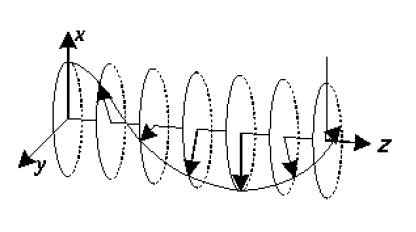
\includegraphics[scale = 0.6]{2.png}
}
\centerline{Figure 1. Elliptically polarized light propagating in the $z$ direction.} 
\centerline{The light is polarized in the $xy$ plane.}

Polarizer is a device used to produce polarized light. It polarizes the light using the principle 
of dichroism: a selective absorption mechanism tends to allow the light polarized in a certain
direction to pass through the material, while the light polarized in all other directions is absorbed. This
turns the incident natural light into a linearly polarized. A polarization device can also be used to detect and
analyze linearly polarized, natural and partialy polarized light (it is then called an analyzer)

Malus' law says that the light coming out of a polarization device is a change of the light brightness. 
Suppose that we have two polarizers arranged parallel (a polarizer and an analyzer). Let the angle between 
their transmission directions be $\theta$. The light is incident normally on the polarizer 
and then continues to the analizer. The intensity of the linearly polarized light leaving the 
analyzer is

\centerline{
	\begin{math}
		I_{light} = I_{light,0} \cos^2\theta
	\end{math}
}

\noindent where $ I_{light,0} $ is the intensity of the linearly polarized light incident 
on the analyzer.

For a single polarizer, if a polarized light is incident on it, then the transmitted light intensity 
will change periodically when rotating the polarizer. If the incident light is partially or elliptically 
polarized, the minimum intensity will not be zero as there will be always some component of the light 
polarized in the transmission direction. The incident light must be natural or circularly polarized 
if the intensity does not change at all. Hence, by using a polarizer, one can distinguish linearly polarized 
light from the natural and circularly polarized light.




\section{Experimental setup}

The measurement setup is composed of: a semiconductor laser, a tungsten iodine lamp, 
a silicon photo-cell, a UT51 digital universal meter, as well as two polarizers, 1/2-wave 
and 1/4-wave plates and a lens with a glass sheet. The elements are placed on an optical bench.

The uncertainty of the wave plates are 2$^{\circ}$, and the uncertainty for silicon photo-cell is 0.001$\mu$A.

\centerline{
	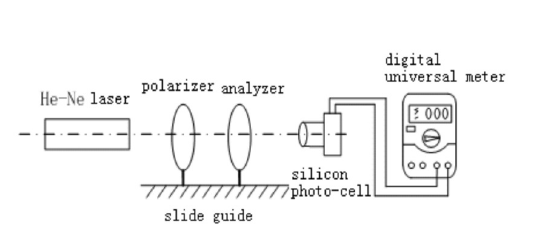
\includegraphics[scale = 0.6]{5.png}
}

\centerline{Figure 2. Experimental setup for a demonstration of Malus' law.}


\section{Measurements}
\subsection{Demonstration of Malus' Law}
\begin{enumerate}
	\item Assemble the measurement setup according to Figure 2. Make sure the laser 
passes through the polarizer first.
	\item Rotate the analyzer for 360$^{\circ}$ and observe the change in light intensity 
to find the maximus elctric current $I_0$.
	\item Set the analyzer to $90^{\circ}$ amd adjust the polarizer until the elctric current reaches minimum.
	\item Rotate the analyzer from $90^{\circ}$ to $0^{\circ}$ and record the magnitude of current $I$ every 
$5^{\circ}$. Record the values in a table and plot the graph $I/I_0$ s. $\cos^2 \theta$.
\end{enumerate}

\subsection{Linearly Polarized Light and the Half-wave Plate}
\centerline{
	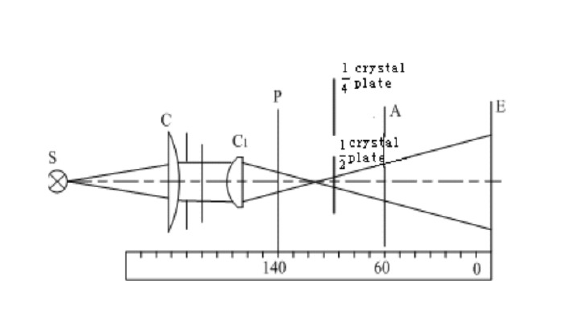
\includegraphics[scale = 0.6]{6.png}
}
\centerline{Figure 3. Experimental setup for the 1/2-wave plate.}

\begin{enumerate}
	\item Set up the equipment on the optical bench according to Figure 3. Make the analizer and the polarizer 
perpendicular to each other, so that the extinction of light can be observed on screen.
	\item Insert the 1/2-wave plate and rotate it to make the light extinction appear again. Let it be the initial position.
	\item Increase the 1/2-wave plate degree by 10$^{\circ}$ each time, then rotate the analyzer to make the 
light extinction appear again. Record the rotation angle of analyzer $\Delta\theta$ in a table.
\end{enumerate}

\subsection{Circularly and Elliptically Polarized Light and the 1/4-wave Plate}

\begin{enumerate}
	\item Set up the equipment on the optical bench according to Figure 3. Make the analizer and the polarizer 
perpendicular to each other, so that the extinction of light can be observed on screen. At this time 
$\theta = 90^{\circ}$
	\item Insert the 1/4-wave plate and rotate it to make the extinction of the light observed on screen again. This is the initial 
position and $\alpha=90^{\circ}$ 
	\item Rotate the analyzer for 360$^{\circ}$ and record the light intensity for every 10$^{\circ}$. Record the data in a table.
	\item Rotate the 1/4-wave plate to $\alpha = 20^{\circ}$ and $\alpha = 45^{\circ}$ and repeat the previous step.
\end{enumerate}
\section{Results}
Uncertainty of $\theta$ is $2^{\circ}$

\subsection{Demonstration of Malus' Law}
\centerline{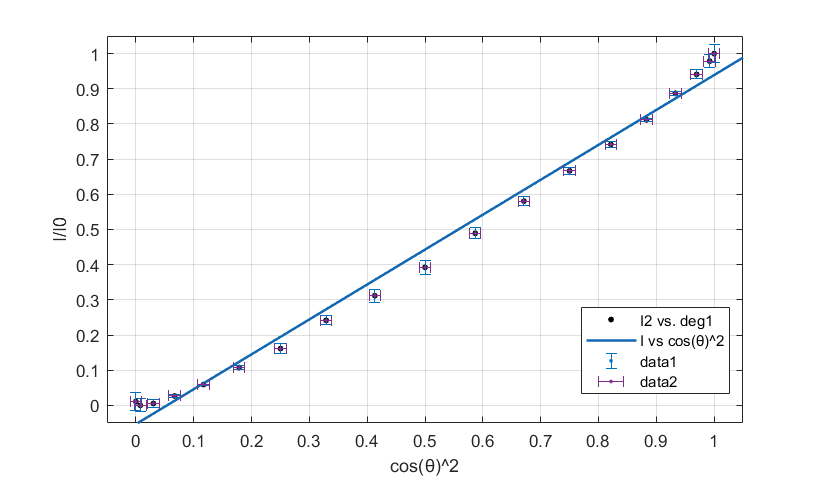
\includegraphics[scale = 0.6]{fig1.png}}
\centerline{Figure 4. Fit graph for experiment 4.1}

The fitting result is:
$$
	k = \frac{I/I_0}{\cos^2(\theta)} = 0.9921 \pm 0.051
$$

\subsection{Linearly Polarized Light and the Half-wave Plate}

\centerline{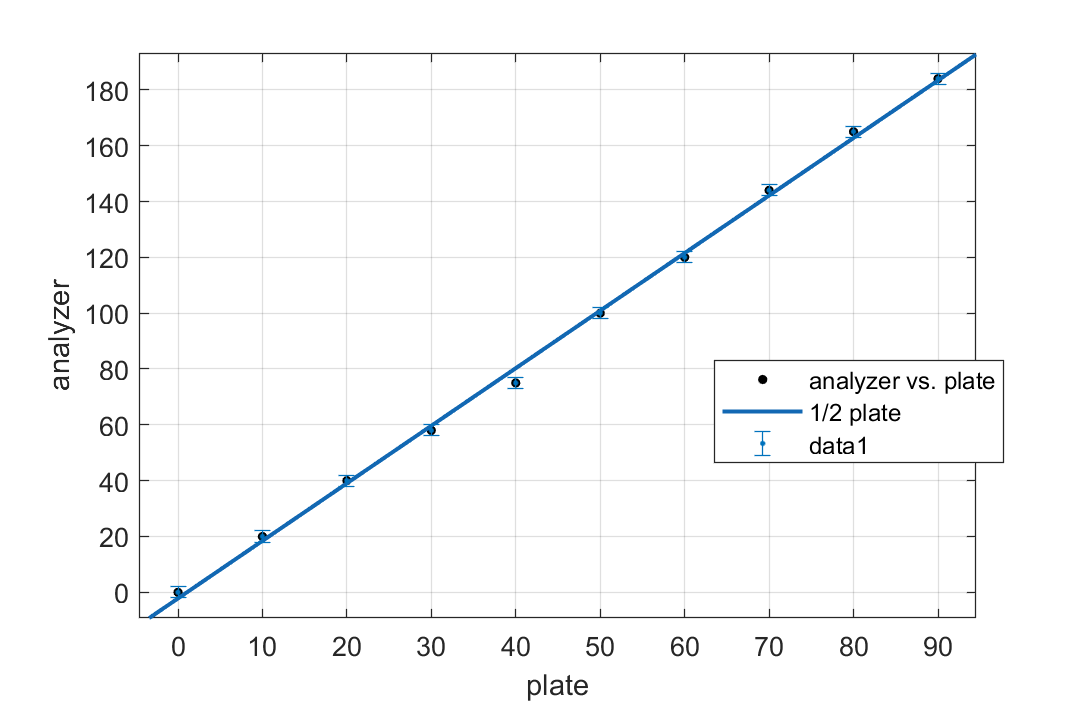
\includegraphics[scale = 0.4]{fig2.png}}
\centerline{Figure 5. Fit graph for experiment 4.2}

The fitting result is:
$$
	k = \frac{\theta_{analyzer}}{\theta_{plate}} = 2.062 \pm 0.064
$$

\subsection{Circularly and Elliptically Polarized Light and the 1/4-wave Plate}

\centerline{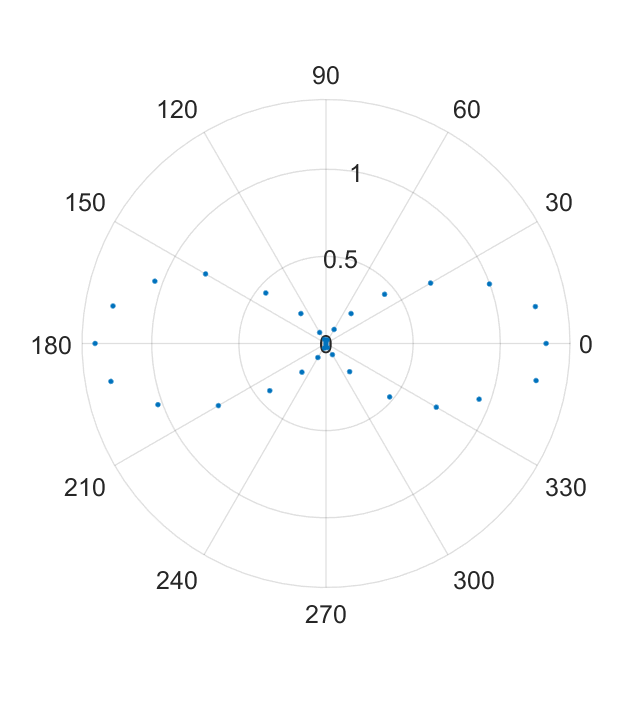
\includegraphics[scale = 0.4]{fig3.png}}
\centerline{Figure 6. Fit graph for experiment 4.3, $\alpha = 0$}

\centerline{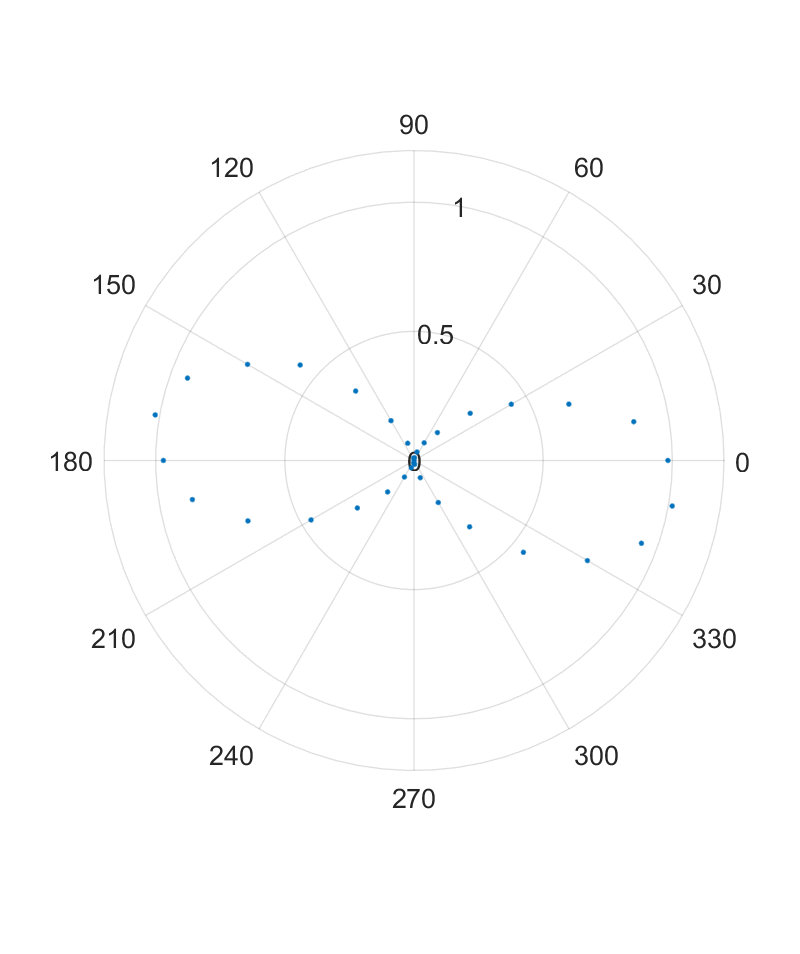
\includegraphics[scale = 0.4]{fig4.png}}
\centerline{Figure 7. Fit graph for experiment 4.3, $\alpha = 20$}

\centerline{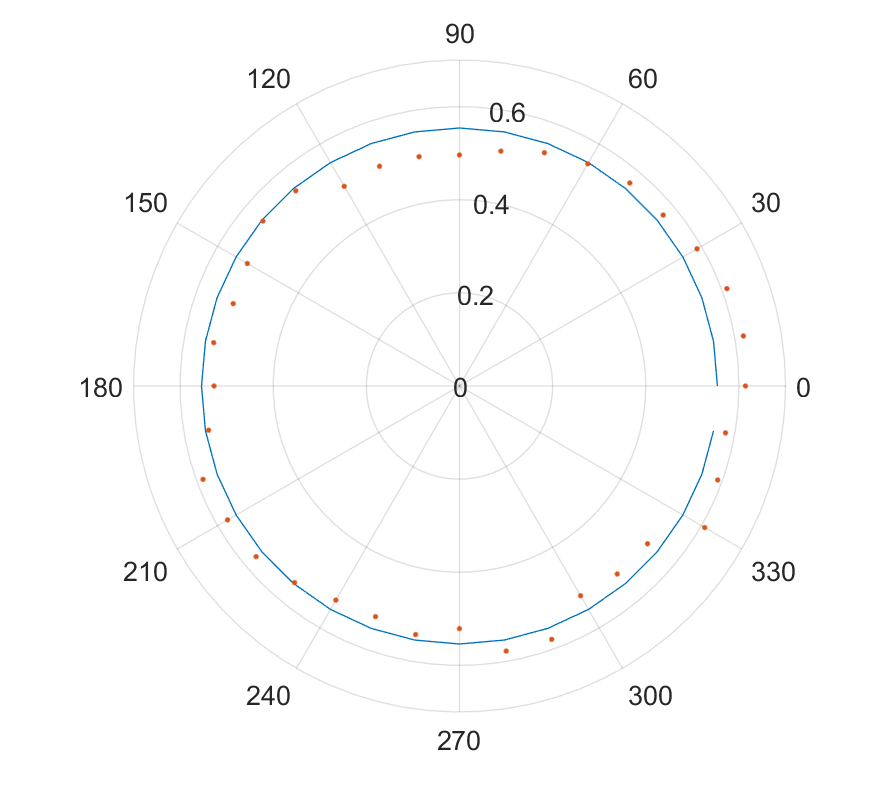
\includegraphics[scale = 0.4]{fig5.png}}
\centerline{Figure 7. Fit graph for experiment 4.3, $\alpha = 45$}

~\\

When $\alpha = 70^{\circ}$:
\begin{table}[!h]
	\begin{center}
	\begin{tabular}{|c|c|}
	\hline
	\multicolumn{2}{|c|}{Rotating angle of the 1/2-wave plate: $70^\circ$}\\
	\hline
	$\theta[^\circ]\pm2[^\circ]$		&	$10^\circ$	\\
	\hline
	$I[\mu A]\pm0.01[\mu A]$	&	1.145	\\
	\hline
	\end{tabular}
	\caption{Measurement data for the 1/2-wave plate ($\alpha = 70^\circ$).}
	\label{tab-0}
	\end{center}
\end{table}

When $\alpha = 20^{\circ}$, $I$ reaches maximum when $\theta_1 = 170^{\circ}$

When $\alpha = 70^{\circ}$, $I$ reaches maximum when $\theta_2 = 10^{\circ}$

So that $\theta_1 + \theta_2 = 180^{\circ} = 90^{\circ}\cdot 2$, which proves the theorem is true.

\section{Uncertainties}
\subsection{Demonstration of Malus' Law}

To calculate the uncertainty of $\cos^(\theta)$, we use the 
uncertainty of $\theta$. Since $u_{\theta}$ is given by $2^{\circ}$:
$$
	u_{\cos^2\theta} = 2\sin\theta\cos\theta u_{\theta}
$$
We can apply this formula to all $\theta$ taken. When $\theta=0^{\circ}$:
$$
	u_{\cos^2 5^{\circ}} = 2 \times \sin(5^{\circ}) \times \cos(5^{\circ}) \times u_{\theta} = 0.3
$$

Here the table lists all the value of $u_{\cos^2\theta}$:

\begin{table}[H]
	\centering
	\begin{tabular}{|l|ll|l|ll|}
	\hline
	$\theta${[}$^{\circ}${]} & \multicolumn{2}{c|}{uncertainty $u_{\cos^2\theta}$} & $\theta${[}$^{\circ}${]} & \multicolumn{2}{c|}{uncertainty $u_{\cos^2\theta}$} \\ \hline
	0°           			 & \multicolumn{1}{l|}{$u_{\cos^2 0^{\circ}}$} 	   & 0     & 50°          & \multicolumn{1}{l|}{$u_{\cos^2 50^{\circ}}$}    & 2.0   \\ \hline
	5°           			 & \multicolumn{1}{l|}{$u_{\cos^2 5^{\circ}}$}     & 0.3   & 55°          & \multicolumn{1}{l|}{$u_{\cos^2 55^{\circ}}$}    & 1.9   \\ \hline
	10°          			 & \multicolumn{1}{l|}{$u_{\cos^2 10^{\circ}}$}    & 0.7   & 60°          & \multicolumn{1}{l|}{$u_{\cos^2 60^{\circ}}$}    & 1.7   \\ \hline
	15°          			 & \multicolumn{1}{l|}{$u_{\cos^2 15^{\circ}}$}    & 1.0   & 65°          & \multicolumn{1}{l|}{$u_{\cos^2 65^{\circ}}$}    & 1.5   \\ \hline
	20°          			 & \multicolumn{1}{l|}{$u_{\cos^2 20^{\circ}}$}    & 1.3   & 70°          & \multicolumn{1}{l|}{$u_{\cos^2 70^{\circ}}$}    & 1.3   \\ \hline
	25°          			 & \multicolumn{1}{l|}{$u_{\cos^2 25^{\circ}}$}    & 1.5   & 75°          & \multicolumn{1}{l|}{$u_{\cos^2 75^{\circ}}$}    & 1.0   \\ \hline
	30°          			 & \multicolumn{1}{l|}{$u_{\cos^2 30^{\circ}}$}    & 1.7   & 80°          & \multicolumn{1}{l|}{$u_{\cos^2 80^{\circ}}$}    & 0.7   \\ \hline
	35°          			 & \multicolumn{1}{l|}{$u_{\cos^2 35^{\circ}}$}    & 1.9   & 85°          & \multicolumn{1}{l|}{$u_{\cos^2 85^{\circ}}$}    & 0.3   \\ \hline
	40°          			 & \multicolumn{1}{l|}{$u_{\cos^2 40^{\circ}}$}    & 2.0   & 90°          & \multicolumn{1}{l|}{$u_{\cos^2 90^{\circ}}$}    & 0     \\ \hline
	45°          			 & \multicolumn{1}{l|}{$u_{\cos^2 45^{\circ}}$}    & 2.0   &              & \multicolumn{1}{l|}{}    &       \\ \hline
	\end{tabular}
	\caption{Uncertainty of $\cos\theta$}
	\label{tab-1}
\end{table}

The uncertainty of $I/I_0$ can be found by applying the uncertainty propagation formula

\begin{align*}
	u_{I/I_0}&=\sqrt{\left(\frac{\partial I/I_0}{\partial I}\right)^2u_{I}^2+\left(\frac{\partial I/I_0}{\partial I_0}\right)^2u_{I_0}^2}\\
	&=\sqrt{\left(\frac{1}{I_0}\right)^2u_{I}^2+\left(\frac{I}{I_0^2}\right)^2u_{I_0}^2}\\
\end{align*}

Since $u_I = u_{I_0} = 0.001 \mu A$ and $I_0 = 1.860 \mu A$, when $\theta = 0^{\circ}$ and $I = 1.860 \mu A$:
$$
	u_{I/I_0} = \sqrt{\left(\frac{1}{1.860}\right)^2 0.001^2+\left(\frac{1.860}{1.860^2}\right)^2 0.001^2} = 0.0011
$$

Here the table lists all the value of $u_{I/I_0}$:

\begin{table}[H]
	\centering
	\begin{tabular}{|l|cl|l|cl|}
	\hline
	I {[}$\mu A${]} & \multicolumn{2}{c|}{uncertainty   $u_{I/I_0}$} & I {[}$\mu A${]} & \multicolumn{2}{c|}{uncertainty $u_{I/I_0}$} \\ \hline
	1.860      & \multicolumn{2}{c|}{0.0011}                    & 0.580      & \multicolumn{2}{c|}{0.0006}                  \\ \hline
	1.820      & \multicolumn{2}{c|}{0.0011}                    & 0.450      & \multicolumn{2}{c|}{0.0006}                  \\ \hline
	1.750      & \multicolumn{2}{c|}{0.0011}                    & 0.300      & \multicolumn{2}{c|}{0.0006}                  \\ \hline
	1.650      & \multicolumn{2}{c|}{0.0010}                    & 0.200      & \multicolumn{2}{c|}{0.0005}                  \\ \hline
	1.510      & \multicolumn{2}{c|}{0.0010}                    & 0.110      & \multicolumn{2}{c|}{0.0005}                  \\ \hline
	1.380      & \multicolumn{2}{c|}{0.0009}                    & 0.050      & \multicolumn{2}{c|}{0.0005}                  \\ \hline
	1.240      & \multicolumn{2}{c|}{0.0009}                    & 0.010      & \multicolumn{2}{c|}{0.0005}                  \\ \hline
	1.080      & \multicolumn{2}{c|}{0.0008}                    & 0.000      & \multicolumn{2}{c|}{0.0005}                  \\ \hline
	0.910      & \multicolumn{2}{c|}{0.0007}                    & 0.020      & \multicolumn{2}{c|}{0.0005}                  \\ \hline
	0.730      & \multicolumn{2}{c|}{0.0007}                    &            & \multicolumn{2}{c|}{}                        \\ \hline
	\end{tabular}
	\caption{Uncertainty of $u_{I/I_0}$}
	\label{tab-2}
	\end{table}

\subsection{Linearly Polarized Light and the Half-wave Plate}
The uncertainty for all the data is:
\begin{align*}
	&u_\theta = 2^{\circ}\\
	&u_{\Delta\theta} = 2^{\circ}
\end{align*}

\subsection{Circularly and Elliptically Polarized Light and the 1/4-wave Plate}
To calculate the uncertainty for $\sqrt{I/I_0}$, we can calculate the partial derivative:

\[
\begin{aligned}
	u_{I^{0.5} / I^{0.5}_{0}} &=\sqrt{\left(\frac{\partial I^{0.5} / I^{0.5}_{0}}{\partial I}\right)^{2} u_{I}^{2}+\left(\frac{\partial I^{0.5} / I^{0.5}_{0}}{\partial I_{0}}\right)^{2} u_{I_{0}}^{2}} \\
	&=0.5*\sqrt{\frac{1}{I \cdot I_0} u_{I}^{2}+\frac{I}{I_{0}^{3}} u_{I_{0}}^{2}}
\end{aligned}
\]

When $I = 1.263 \mu A$ and $I_0 = 1.325 \mu A$:
\[
\begin{aligned}
	u_{I^{0.5} / I^{0.5}_{0}}=0.5*\sqrt{\frac{1}{1.263\times1.325} 0.001^{2}+\frac{1.263}{1.325^{3}} 0.001^{2}} = 0.0005
\end{aligned}
\]

Here the table lists all the value of $u_{I^{0.5} / I^{0.5}_{0}}$:


When $\alpha = 0^{\circ}$:
\begin{table}[H]
	\centering
	\begin{tabular}{|l|cl|l|cl|}
	\hline
	$(I/I_0)^{0.5}$ & \multicolumn{2}{c|}{uncertainty   $u_{I^{0.5}/I_0^{0.5}}$} & $(I/I_0)^{0.5}$ & \multicolumn{2}{c|}{uncertainty   $u_{I^{0.5}/I_0^{0.5}}$} \\ \hline
	0.976323        & \multicolumn{2}{c|}{0.0005}                                & 1.000000        & \multicolumn{2}{c|}{0.0005}                                \\ \hline
	0.959560        & \multicolumn{2}{c|}{0.0005}                                & 0.972451        & \multicolumn{2}{c|}{0.0005}                                \\ \hline
	0.867875        & \multicolumn{2}{c|}{0.0005}                                & 0.879966        & \multicolumn{2}{c|}{0.0005}                                \\ \hline
	0.723200        & \multicolumn{2}{c|}{0.0006}                                & 0.733562        & \multicolumn{2}{c|}{0.0006}                                \\ \hline
	0.575605        & \multicolumn{2}{c|}{0.0007}                                & 0.563681        & \multicolumn{2}{c|}{0.0007}                                \\ \hline
	0.411165        & \multicolumn{2}{c|}{0.0009}                                & 0.402820        & \multicolumn{2}{c|}{0.0009}                                \\ \hline
	0.264931        & \multicolumn{2}{c|}{0.0014}                                & 0.264931        & \multicolumn{2}{c|}{0.0014}                                \\ \hline
	0.128856        & \multicolumn{2}{c|}{0.0029}                                & 0.145369        & \multicolumn{2}{c|}{0.0026}                                \\ \hline
	0.047583        & \multicolumn{2}{c|}{0.0079}                                & 0.047583        & \multicolumn{2}{c|}{0.0079}                                \\ \hline
	0.027472        & \multicolumn{2}{c|}{0.0137}                                & 0.027472        & \multicolumn{2}{c|}{0.0137}                                \\ \hline
	0.047583        & \multicolumn{2}{c|}{0.0079}                                & 0.038851        & \multicolumn{2}{c|}{0.0097}                                \\ \hline
	0.137361        & \multicolumn{2}{c|}{0.0027}                                & 0.137361        & \multicolumn{2}{c|}{0.0027}                                \\ \hline
	0.234722        & \multicolumn{2}{c|}{0.0016}                                & 0.236324        & \multicolumn{2}{c|}{0.0016}                                \\ \hline
	0.411165        & \multicolumn{2}{c|}{0.0009}                                & 0.399055        & \multicolumn{2}{c|}{0.0010}                                \\ \hline
	0.583419        & \multicolumn{2}{c|}{0.0007}                                & 0.600000        & \multicolumn{2}{c|}{0.0007}                                \\ \hline
	0.776057        & \multicolumn{2}{c|}{0.0006}                                & 0.742764        & \multicolumn{2}{c|}{0.0006}                                \\ \hline
	0.888076        & \multicolumn{2}{c|}{0.0005}                                & 0.840036        & \multicolumn{2}{c|}{0.0005}                                \\ \hline
	0.967783        & \multicolumn{2}{c|}{0.0005}                                & 0.961131        & \multicolumn{2}{c|}{0.0005}                                \\ \hline
	\end{tabular}
	\caption{Uncertainty of $u_{I^{0.5} / I^{0.5}_{0}}$ when $\alpha = 0^{\circ}$}
	\label{tab-3}
\end{table}

When $\alpha = 20^{\circ}$:
\begin{table}[H]
	\centering
	\begin{tabular}{|l|cl|l|cl|}
	\hline
	$(I/I_0)^{0.5}$ & \multicolumn{2}{c|}{uncertainty   $u_{I^{0.5}/I_0^{0.5}}$} & $(I/I_0)^{0.5}$ & \multicolumn{2}{c|}{uncertainty   $u_{I^{0.5}/I_0^{0.5}}$} \\ \hline
	0.983142        & \multicolumn{2}{c|}{0.0007}                                & 0.976619        & \multicolumn{2}{c|}{0.0007}                                \\ \hline
	0.921714        & \multicolumn{2}{c|}{0.0007}                                & 0.925441        & \multicolumn{2}{c|}{0.0007}                                \\ \hline
	0.792045        & \multicolumn{2}{c|}{0.0007}                                & 0.820101        & \multicolumn{2}{c|}{0.0007}                                \\ \hline
	0.654010        & \multicolumn{2}{c|}{0.0008}                                & 0.672540        & \multicolumn{2}{c|}{0.0008}                                \\ \hline
	0.528444        & \multicolumn{2}{c|}{0.0010}                                & 0.530301        & \multicolumn{2}{c|}{0.0010}                                \\ \hline
	0.372348        & \multicolumn{2}{c|}{0.0013}                                & 0.395401        & \multicolumn{2}{c|}{0.0013}                                \\ \hline
	0.278710        & \multicolumn{2}{c|}{0.0018}                                & 0.269746        & \multicolumn{2}{c|}{0.0018}                                \\ \hline
	0.185513        & \multicolumn{2}{c|}{0.0027}                                & 0.171751        & \multicolumn{2}{c|}{0.0029}                                \\ \hline
	0.104001        & \multicolumn{2}{c|}{0.0047}                                & 0.099161        & \multicolumn{2}{c|}{0.0050}                                \\ \hline
	0.044346        & \multicolumn{2}{c|}{0.0111}                                & 0.044346        & \multicolumn{2}{c|}{0.0111}                                \\ \hline
	0.099161        & \multicolumn{2}{c|}{0.0050}                                & 0.121447        & \multicolumn{2}{c|}{0.0040}                                \\ \hline
	0.264222        & \multicolumn{2}{c|}{0.0019}                                & 0.264222        & \multicolumn{2}{c|}{0.0019}                                \\ \hline
	0.418359        & \multicolumn{2}{c|}{0.0012}                                & 0.429950        & \multicolumn{2}{c|}{0.0012}                                \\ \hline
	0.587480        & \multicolumn{2}{c|}{0.0009}                                & 0.573934        & \multicolumn{2}{c|}{0.0009}                                \\ \hline
	0.751923        & \multicolumn{2}{c|}{0.0008}                                & 0.737398        & \multicolumn{2}{c|}{0.0008}                                \\ \hline
	0.855315        & \multicolumn{2}{c|}{0.0007}                                & 0.872952        & \multicolumn{2}{c|}{0.0007}                                \\ \hline
	0.957812        & \multicolumn{2}{c|}{0.0007}                                & 0.959863        & \multicolumn{2}{c|}{0.0007}                                \\ \hline
	1.000000        & \multicolumn{2}{c|}{0.0007}                                & 0.999016        & \multicolumn{2}{c|}{0.0007}                                \\ \hline
	\end{tabular}
	\caption{Uncertainty of $u_{I^{0.5} / I^{0.5}_{0}}$ when $\alpha = 20^{\circ}$}
	\label{tab-4}
	\end{table}
	



When $\alpha = 70^{\circ}$:
\begin{table}[H]
	\centering
	\begin{tabular}{|l|cl|l|cl|}
	\hline
	$(I/I_0)^{0.5}$ & \multicolumn{2}{c|}{uncertainty   $u_{I^{0.5}/I_0^{0.5}}$} & $(I/I_0)^{0.5}$ & \multicolumn{2}{c|}{uncertainty   $u_{I^{0.5}/I_0^{0.5}}$} \\ \hline
	0.995953        & \multicolumn{2}{c|}{0.0007}                                & 0.922699        & \multicolumn{2}{c|}{0.0008}                                \\ \hline
	1.000000        & \multicolumn{2}{c|}{0.0007}                                & 0.940044        & \multicolumn{2}{c|}{0.0008}                                \\ \hline
	0.993517        & \multicolumn{2}{c|}{0.0007}                                & 0.972979        & \multicolumn{2}{c|}{0.0007}                                \\ \hline
	0.975466        & \multicolumn{2}{c|}{0.0007}                                & 0.963804        & \multicolumn{2}{c|}{0.0008}                                \\ \hline
	0.960446        & \multicolumn{2}{c|}{0.0008}                                & 0.959604        & \multicolumn{2}{c|}{0.0008}                                \\ \hline
	0.958762        & \multicolumn{2}{c|}{0.0008}                                & 0.943475        & \multicolumn{2}{c|}{0.0008}                                \\ \hline
	0.943475        & \multicolumn{2}{c|}{0.0008}                                & 0.926194        & \multicolumn{2}{c|}{0.0008}                                \\ \hline
	0.927937        & \multicolumn{2}{c|}{0.0008}                                & 0.922699        & \multicolumn{2}{c|}{0.0008}                                \\ \hline
	0.909473        & \multicolumn{2}{c|}{0.0008}                                & 0.935738        & \multicolumn{2}{c|}{0.0008}                                \\ \hline
	0.895149        & \multicolumn{2}{c|}{0.0008}                                & 0.917431        & \multicolumn{2}{c|}{0.0008}                                \\ \hline
	0.898752        & \multicolumn{2}{c|}{0.0008}                                & 0.966315        & \multicolumn{2}{c|}{0.0008}                                \\ \hline
	0.900547        & \multicolumn{2}{c|}{0.0008}                                & 0.967150        & \multicolumn{2}{c|}{0.0007}                                \\ \hline
	0.894247        & \multicolumn{2}{c|}{0.0008}                                & 0.916550        & \multicolumn{2}{c|}{0.0008}                                \\ \hline
	0.940044        & \multicolumn{2}{c|}{0.0008}                                & 0.922699        & \multicolumn{2}{c|}{0.0008}                                \\ \hline
	0.943475        & \multicolumn{2}{c|}{0.0008}                                & 0.922699        & \multicolumn{2}{c|}{0.0008}                                \\ \hline
	0.921823        & \multicolumn{2}{c|}{0.0008}                                & 0.991075        & \multicolumn{2}{c|}{0.0007}                                \\ \hline
	0.913903        & \multicolumn{2}{c|}{0.0008}                                & 0.976294        & \multicolumn{2}{c|}{0.0007}                                \\ \hline
	0.930544        & \multicolumn{2}{c|}{0.0008}                                & 0.967985        & \multicolumn{2}{c|}{0.0007}                                \\ \hline
	\end{tabular}
	\caption{Uncertainty of $u_{I^{0.5} / I^{0.5}_{0}}$ when $\alpha = 70^{\circ}$}
	\label{tab-5}
	\end{table}

\newpage

\section{Conclusions and discussion}
In this lab, we studied and experimented on the light polarization phenomenon and verify Malus' law, the way 1/2 and 1/4-wave plates work in optical systems and generation and detection of elliptically and circularly polarized light.\\

This effect can be visible since the light coming out of a polarization device is a change of the light brightness. It can be represented by the intensity of elctric flow:

$$I_{light}=I_{light,0}cos^2\theta$$

Since the amplitudes of the o-wave and the e-wave are both functions of $ \alpha $, the polarization state after passing through a 1/4-wave plate depends on the angle:\\

When $ \alpha= 0 $, the transmitted light is linearly polarized with the polarization axis parallel to the optical axis of the 1/4-wave plate;

When $ \alpha=\pi/2 $, the transmitted light is linearly polarized with the polarization axis perpendicular to the optical axis of the 1/4-wave plate;

When $ \alpha=\pi/4 $, the transmitted light is circularly polarized;

Otherwise, the transmitted light is elliptically polarized.

~\\
\indent In this experiment, the error and inaccuracies mainly come from system errors. 
Moreover, the 1/4-wave plate we used seemed to have a little problem and is inaccurate. We 
didn't notice this problem until we were setting $\alpha = 45$. So, the measurement of $\alpha = 20$ 
might be inaccurate.


\section{References}
    \begin{enumerate}
        \item Qin Tian, Cao Jianjun, Yi Hankun, Wu Ziyou, Zhang Yifei, Yao Yuan, Mateusz Krzyzosiak
    \end{enumerate}

\end{document}
